\documentclass[12pt,oneside]{article}

% packages
\usepackage[ngerman]{babel}
\usepackage[hidelinks]{hyperref}
\usepackage{adjustbox}
\usepackage{graphicx}
\usepackage{xcolor}

% global config
\newcommand{\gqq}[1]{\glqq{#1}\grqq}

\hypersetup{
	colorlinks,
	linkcolor = {red!60!black},
	citecolor = {blue!50!black},
	urlcolor = {blue!70!black},
}


\begin{document}


\title{
	Optimierung von Voxel Engines
	\\ mittels Culling und Greedy Meshing
	\\ \large{MINT Hausarbeit an der Martin Luther Schule}
}
\author{Arne Daude}
\maketitle

\tableofcontents

\pagebreak


\section{Einleitung}

Eine Voxel Engine ist zuständig Voxels auf den
Bildschirm zu projizieren. Voxels sind dabei wie
Pixel, nur 3D (der Name \gqq{Voxel} kommt von
\gqq{Volumen} kombiniert mit \gqq{Pixel}).
Also werden viele kleine Würfel zusammengesetzt,
um ein drei dimensionale Objekt darzustellen.

Dies wird in manchen Videospielen benutzt, wie
Minecraft. Als Spieleentwickler erstelle ich auch
ein Voxel Spiel und bin auf das Problem getreten,
wie man diese implementiert.
Es gibt hauptsächlich zwei Varianten,
wie Voxel Engines implementiert werden:

\begin{itemize}
	\item Volumengrafik:
	Es wird ein komplett neues Verfahren entwickelt,
	um die Voxels zu rendern, welches direkt mit
	den Voxels arbeitet. Dies hat zwar gute
	Performance, hat aber auch die Limitation,
	dass alle Voxel nur einfache Würfel seien können.

	\item Polygon Meshes:
	Die Voxels werden zuerst in ein 3D Mesh von
	Dreiecken (oder allgemein Polygonen) umgewandelt
	und dann von einem typischen 3D Renderer angezeigt.
	Somit muss man keinen neuen Renderer erstellen und
	kann auch andere Modelle als nur Würfel anzeigen,
	aber dieses Verfahren hat dafür schlechtere
	Performance.
\end{itemize}

Wegen der einfacheren Implementation, und dass man
komplexere Modelle als nur Würfel erstellen kann,
werden in den meisten Spielen die Polygon Mesh
Variante bevorzugt.

\begin{figure}[ht]
	\begin{minipage}[c]{0.48\textwidth}
Mit der Polygon Meshes Implementation sieht dann ein
Voxel wie rechts gezeigt aus.
Die grünen Linien zeigen dabei wie es in Dreiecke
eingeteilt ist.
	\end{minipage}
	\begin{minipage}[c]{0.5\textwidth}
		\begin{center}
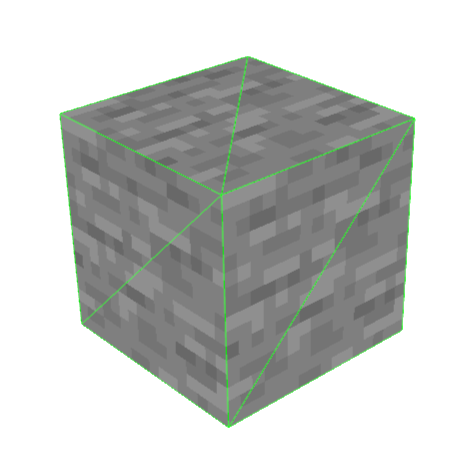
\includegraphics[width=0.8\textwidth]{assets/SingleVoxel.png}
		\end{center}
	\end{minipage}\hfill
\end{figure}

\goodbreak

Ein Quadrat wird aus $2$ Dreiecken zusammengesetzt
und ein Würfel hat $6$ Seiten. Somit besteht ein Würfel
aus $12$ Dreiecken. Wenn der Spieler nur $100$ Voxels
weit sehen könnte, wäre der Durchmesser $200$ Voxels
und somit das gesamte Volumen das angezeigt werden
muss $200^3 = 8.000.000$ Voxels groß, also
$12 \cdot 200^3 = 96.000.000$ Dreiecke.

Wir sehen also, dass schon bei einer sehr kleinen
Sichtweite sehr viele Dreiecke erstellt werden.
Diese Hausarbeit beschäftigt sich deswegen mit der
Optimierung die Anzahl der Dreiecke so weit wie
möglich zu reduzieren.


\section{Culling}

% TODO


\section{Greedy Meshing}

% TODO

{ \subsection{Erste Implementation}

% TODO
 }

{ \subsection{Binäres Greedy Meshing}

% TODO
 }

{ \subsection{Korrektur der Texturen}

% TODO
 }


\section{Fazit}

% TODO


\section{Literaturverzeichnis}

% TODO


% TODO end text with inserted signature


\end{document}
